\chapter{Problemanalyse} \label{Problemanalyse}
Det følgende afsnit har til formål at afdække anvendelse og fremstilling af speckle patterns til brug ved DIC, herunder undersøgelse af hvilke parametre, der beskriver et optimalt speckle pattern. Derefter defineres og undersøges robotter for at opnå den nødvendige forståelse for deres mekanismer, så en løsning til fremstilling af speckle patterns kan udvikles.

% --- DIC ---
\section{Digital Image Correlation} \label{DIC afsnit}
DIC er en optisk metode, der anvender digitale billeder til at måle deformation, bevægelse og tøjning i materialer. DIC fungerer ved at sammenligne billeder taget før, under og efter deformation for at måle forskydninger og udregne tøjninger. Metoden gør det muligt at undersøge deformationer over hele emnet og omkring revner. (\cite{Zaya2023ApplicationReview})

\begin{figure}[H]
    \centering
    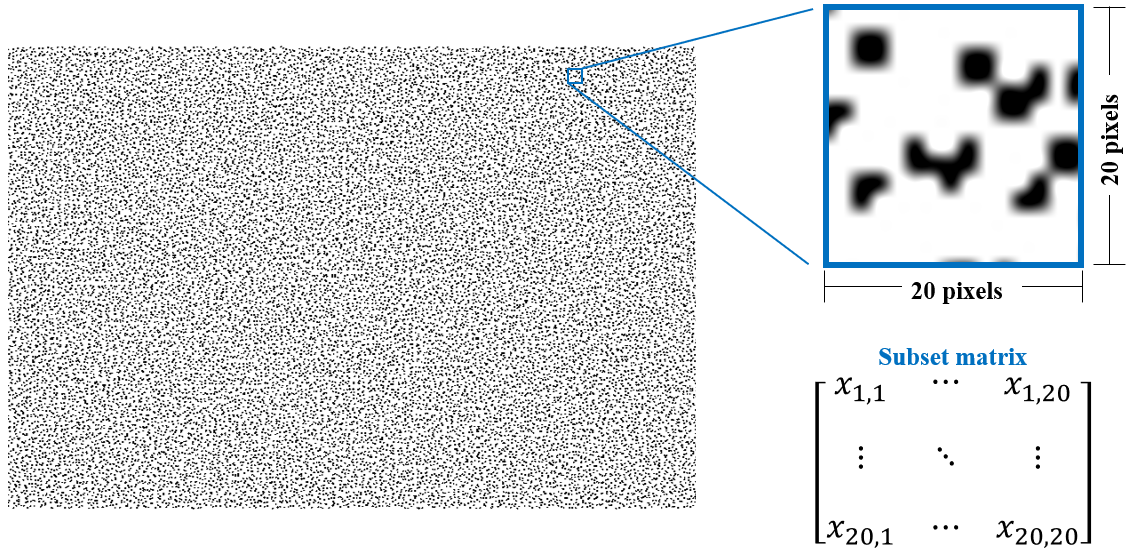
\includegraphics[width=0.85\linewidth]{Sections/2 Problemanalyse/Media/Speckle pattern subset matrix.png}
    \caption{Illustration af speckles pattern, i øverste højre hjørne ses et subset på $20 \times 20 \text{pixels}$ . Det er genereret med software fra Correlated Solutions (\cite{CorrelatedSolutions2025SpeckleInc.})}
    \label{fig:speckle pattern subset}
\end{figure} \plainbreak{-0.5}

DIC starter med et reference billede taget før deformation, eventuelt efterfulgt af billeder taget under deformationsprocessen, samt et billedet efter deformation. Computersoftware bruger forskellen mellem referencebilledet og de efterfølgende billeder, til at finde deformationer, som herefter udregnes til tøjninger i prøven. Softwaren gør dette ved at identificere subsets af pixels (se figur \ref{fig:speckle pattern subset}) i reference billedet, og derefter finder samme deformerede subset på billedet hvor emnet er deformeret. (\cite{Zaya2023ApplicationReview})

DIC benyttes både til undersøgelser af plane emner (2D), samt rumlige emner (3D). I 2D undersøgelser må materialet ikke deformere sig ud af planet, da denne bevægelse ikke kan blive set af kameraet. 3D DIC benytter sig af to eller flere kameraer, og er optimal i situationer, hvor et materiale bevæger sig fra planet til rummet (figur \ref{fig:2D og 3D DIC}).

\begin{figure}[H]
    \centering
    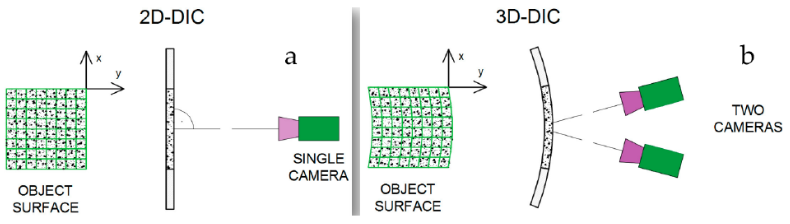
\includegraphics[width=0.9\linewidth]{Sections/2 Problemanalyse/Media/DIC 2D eller 3D.png}
    \caption{Opstilling af 2D og 3D digital image correlation (\cite{Wang2023FiberMonitoring})}
    \label{fig:2D og 3D DIC}
\end{figure} \plainbreak{-0.5}

Opstillingen med flere kameraer giver mulighed for, at tage flere billeder fra forskellige vinkler, og ved hjælp af stereo triangulering, danne en 3D model af objektet. (\cite{Byrne2020DigitalSoftware})


Speckle patterns opdeles i denne rapport i to dele, mikro- og makroskala. I denne rapport defineres mikroskala som den størrelse, der ikke kan opfanges med det blotte øje, og makroskala er den størrelse, der kan fanges med det blotte øje. Der vælges at arbejde i makroskala, med prikker ned til \SI{0,1}{mm} i diameter, fordi det vurderes, at være realistisk at lave speckle patterns i en størrelsesorden man kan se, og ikke mindre.


%Vinklen mellem to kameraer og objektet kaldes stereo vinklen. Denne vinkel kan justeres afhængig af ønsket resultat. Hvis man ønsker større undersøgelse rettet mod et plan, kan vinklen mindskes, og til en rumlig undersøgelse med bevægelse ud af planet, kan vinklen øges. Den optimale vinkel for 3D DIC er mellem 15\degree og 35\degree. (\cite{Bigger2018ACorrelation}) 



\subsection{Alternative målemetoder}
Alternativerne til DIC er primært strain gauges og ekstensometre. Generelt kan de betegnes som spotmålere, det vil sige de måler over et begrænset område, tilgengæld giver de mere nøjagtige målinger end DIC.

\begin{figure}[H]
    \centering
    \begin{subfigure}{0.48\textwidth}
        \centering
        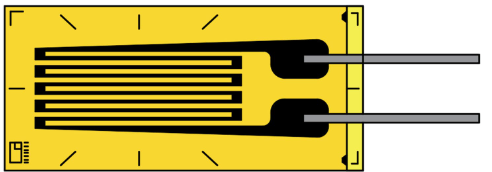
\includegraphics[width=0.8\linewidth]{Sections/2 Problemanalyse/Media/strain gauge.png}
        \caption{Lineær strain gauge der ikke er monteret \parencite{IndustrialQuickSearch2025PrinciplesGauges}}
        \label{fig:straingauge}
    \end{subfigure}
    \begin{subfigure}{0.48\textwidth}
        \centering
        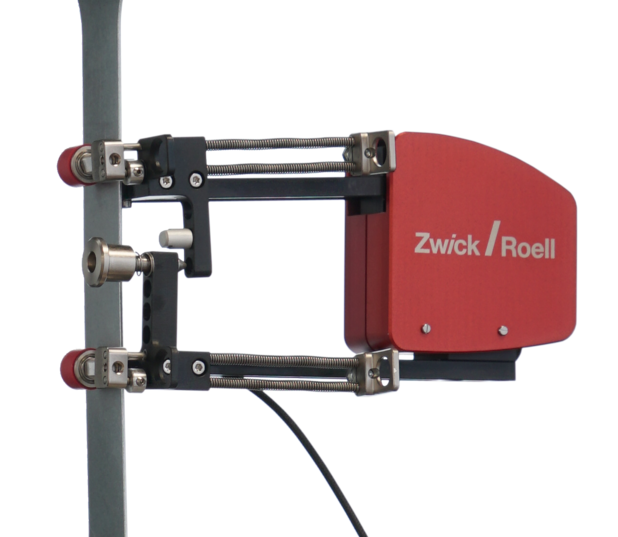
\includegraphics[width=0.7\linewidth]{Sections/2 Problemanalyse/Media/ekstensometer.png}
        \caption{Clip-On ekstensometer monteret \parencite{ZwickRoellExtensometers}}
        \label{fig:ekstensometer}
    \end{subfigure}
    \caption{}
    \label{alternativertildic}
\end{figure} \plainbreak{-0.5}

\textbf{Strain gauges} består af en tynd metalstribe, typisk i zigzaggede parallelle linjer (se figur \ref{fig:straingauge}), på et fleksibelt, isolerende materiale med en form for klistrende underside. Tøjningen findes ved måling af ændringen i modstand, jo mere den deformeres jo højere vil modstanden blive. 

\textbf{Ekstensometre} måler ændringen i afstanden mellem dens to arme, se figur \ref{fig:ekstensometer}. Ekstensiometre kommer i flere varianter der afhænger af,  hvordan armene påsættes emnet.


 

%Siden sin begyndelse i slut 1900-tallet, har DIC gennem årene udviklet sig, og blevet benyttet til en række af forskellige materialeundersøgelser og er blevet til en populær eksperimentel metode blandt andet grundet kosteffektivitet. Materialeundersøgelser som DIC har været igennem inkluderer metaller, polymerer, kompositter, samt biologiske materialer. Disse undersøgelser finder sted på både mikro- og makroskopisk skala, fra millimeter til flere meter. Herved har man også fundet materialer, som ikke er egnet til DIC grundet specifikke faktorer. Nogle af disse inkluderer: Gennemsigtige, bløde eller reflekterende materialer. Løsninger på disse lyder på overfladebelægning af gennemsigtig materiale, benytte speckles af matsort på reflekterende overflader. På bløde materialer er det mere besværligt, men et kamera med en høj rate af billeder i sekundet skal anvendes, grundet skrøbelighed og hurtig deformation. (\cite{Dong2017ACorrelation}; \cite{Bigger2018ACorrelation}) 


% --- Speckle patterns --- 
\plainbreak{2} \section{Speckle pattern} \label{Speckle pattern} 
Speckle patterns er betegnelsen for et billede eller område med prikker, der anvendes til måling af deformationer og tøjninger i materialer ved brug af DIC \parencite{Dong2017ACorrelation}. Prikkerne i et speckle pattern er ikke foruddefineret til at have én bestemt størrelse, form, kontrast, densitet og fordeling. Disse parametre afhænger af størrelsen på emnet der undersøges, kameraets opløsning samt påføringsmetoden. Eksempler på forskellige speckle patterns kan ses i figur \ref{fig:speckle pattern}.\\

\begin{figure}[H]
    \centering
    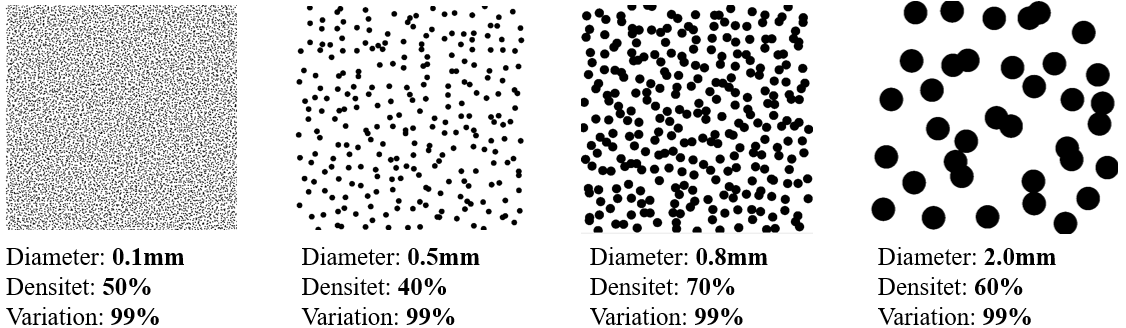
\includegraphics[width=\linewidth]{Sections/2 Problemanalyse/Media/speckle pattern forskellige.png}
    \caption{Eksempler på computergenereret speckle patterns med forskellig densitet og prikstørrelse. Speckle pattern er genereret med software fra Correlated Solutions (\cite{CorrelatedSolutions2025SpeckleInc.})}
    \label{fig:speckle pattern}
\end{figure} \plainbreak{-0.5}

Præcisionen af DIC afhænger blandt andet af det anvendte speckle patterns kvalitet, der kan vurderes ved brug af softwareprogrammer. Programmerne benytter forskellige metoder til kvalitetsvurdering, der vurderer parametre som størrelse, form og fordeling af prikkerne.  
\plainbreak{1} \subsection{Optimale speckle patterns} \label{Optimale speckle patterns}

Et godt speckle pattern er karakteriseret ved høj kontrast mellem prikker og baggrund, og et tilfældigt mønster, der er jævnt fordelt og udgør mellem 50\% og 70\% af billedet. Prikkerne skal have en ensartet radius, samt have en størrelse på mellem $3\times3$ og $5\times5$ pixels. Derudover skal prikkerne være indenfor kameraets field of view (FOV). I denne rapport referer FOV til længden af det område kameraet observerer, det er dermed en konsekvens af dets brændvidde og afstand til emnet. (\cite{Dong2017ACorrelation}; \cite{Su2022Glare:Pattern}; \cite{Gagnon2024ThePatterns}).  


%------
\subsubsection{Høj kontrast}\plainbreak{-0.4} 
DIC benytter gray-level til vurdering af prikkernes placering på overfladen. Gray-level er en grå-skala værdi fra 0\% til 100\%, der beskriver lysintensiteten i et enkelt pixel. Et gray-level på 100\% ses som hvid, hvor 0\% er helt sort, gray-level værdien angiver mængden af lys. Værdierne angives fra 0 til 255 for et 8-bit kamera. Det er nødvendigt med høj kontrast, så kameraet kan opfange forskellen mellem prikker og baggrund. Ofte bruges sorte prikker på hvid baggrund, eller hvide prikker på sort baggrund, idet disse har størst forskel mellem prikkerne og baggrundens gray-level. Forskellen mellem baggrund og prikker skal være på minimum 52 point, for at opnå en optimal værdi, skal denne forskel ligge på 130 point og derover (\cite{Reu2015AllContrast}; \cite{Bigger2018ACorrelation}).


%----- 
\newpage
\subsubsection{Størrelse på prikkerne} \plainbreak{-0.4}
Prikkernes størrelse har betydning for, hvordan prikkerne opfanges af kameraet, samt softwaren bearbejder dataen. For at opnå et optimalt resultat skal prikkerne være større end tre pixels, hvilket afhænger af kameraets opløsning og FOV. Den minimale diameter på prikkerne ($\diameter_{min}$), er derfor afhængig af FOV og antallet af pixels ($n_{pixels}$), som det fremgår af formel \ref{equ:prikstørrelse-Ø_min}. FOV definerer enten bredden eller højden på området, indenfor kameraets synsfelt, der er påført speckle pattern og måles i millimeter. Formlen bruges til at give et estimat, af den minimale diameter prikkerne må have, for at give et optimalt resultat ved DIC. $\diameter_{min}$ beregnes separat for henholdsvis bredden og højden af FOV. Hvis $\diameter_{min}$(bredden) $\neq \diameter_{min}$(højden), benyttes den største diameter (\cite{Reu2014AllAliasing}).
 \begin{equation} \label{equ:prikstørrelse-Ø_min}
     \diameter_{min} = \frac{FOV}{n_{pixels}} \cdot n_{min \ \vee \  max \ pixels} 
 \end{equation}
Prikker mindre end $3\times3$ pixels er vanskelige at bestemme centrum af, idet en prik på $1\times1$ pixels der ligger mellem to pixels vil give en slørret afbildning i gray-level, hvorved kontrasten mellem prik og baggrund mindskes, hvilket medfører en stigning i systematiske fejl. Yderligere øges præcisionen ved brug af prikker over $3\times3$ pixels, fordi det bliver tydeligere på gray-level, hvor prikken er lokaliseret, da den vil dække flere pixels, selvom prikken er placeret mellem to pixels, som det er illusreret på figur \ref{fig:gray-level}. (\cite{Reu2014AllAliasing}; \cite{Cui2024EffectError})

\begin{figure}[H]
    \centering
    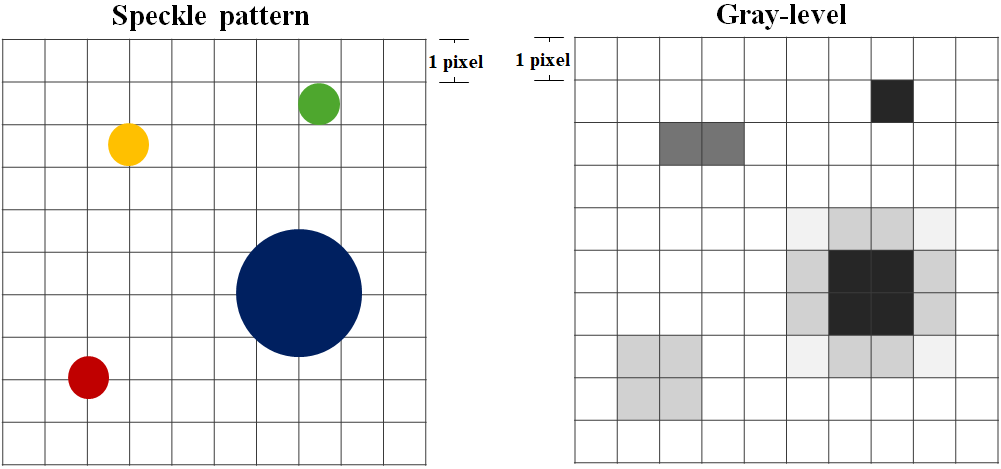
\includegraphics[width=0.8\linewidth]{Sections/2 Problemanalyse/Media/gray-level.png}
    \caption{Illustration af computersoftwares opfattelse af sepckel patterns. Gitteret illustreret et subset på $10\times10$ pixels. Den \textcolor{red}{røde}, \textcolor{greenB}{grønne} og \textcolor{gulny}{gule} prik er alle $1\times1$ pixels, placeret forskelligt i gitteret. Den \textcolor{blue}{blå} prik er $3\times3$ pixels.}
    \label{fig:gray-level}
\end{figure} \plainbreak{-.5}

Prikkerne kan ikke være uendeligt store, da de er begrænset af FOV, kameraets opløsning, det procentvise forhold prikkerne må dække af hele overfladen, samt størrelsen på overfladen der undersøges. Når prikker er større bliver softwaren nød til at gøre brug af tilsvarende større subsets for at garantere unikke subsets. Der skal altså findes et kompromis mellem størrelsen af subsets, dermed nøjagtighed, og systematiske fejl fra prikker placeret på kanten af pixels. Dette kompromis er en prikstørrelse på mellem $5 \times 5$ og $8 \times 8$ pixels. (\cite{Haddadi2008UseTechnique}; \cite{Crammond2013SpeckleCorrelation}; \cite{Dong2017ACorrelation};  \cite{Gagnon2024ThePatterns})


Ved forventning om store deformationer, hvor mindre deformationer er uvæsentlige at undersøge, kan større prikker bruges, uden det har betydning for det der ønskes undersøgt. Overfladens størrelse medvirker til den maksimale størrelse prikkerne kan have, idet store overflader, kan benytte prikker af en større størrelse til subsets, fordi FOV er større (se \ref{equ:prikstørrelse-Ø_min}). Prikkerne i det samme speckle pattern kan variere mellem tre pixels og otte pixels, men for optimal måling skal størrelsesforskellen på prikkerne i det samme speckle pattern holdes minimal(\cite{Crammond2013SpeckleCorrelation}; \cite{Gagnon2024ThePatterns}).  

%-----
\subsubsection{Tilfældigt og isotropt}\plainbreak{-0.4}
Identifikationen af et subset's bevægelse efter deformation af emnet, er kun mulig, hvis prikkerne er arrangeret i et mønster der ikke gentages. Hvis de ligger på linje er det ikke muligt at se hvis prikkerne er forskudt langs den linje (\cite{Zaya2023ApplicationReview}).

%----
\subsubsection{Fordeling af prikkerne}\plainbreak{-0.4}
Et godt speckle pattern har en 50\% til 70\% dækning af prikker. Prikkerne skal være jævnt fordelt med minimum tre pixels mellem alle prikkerne. Hvis prikkerne er for tætte på hinanden, kan softwaren have det vanskeligt med at identificere, om det er én stor prik eller flere små prikker, hvilket øger usikkerheden ved måling. (\cite{Reu2015AllDensity}; \cite{Caliskan2024InvestigationDIC})

\begin{figure}[H]
  \centering
    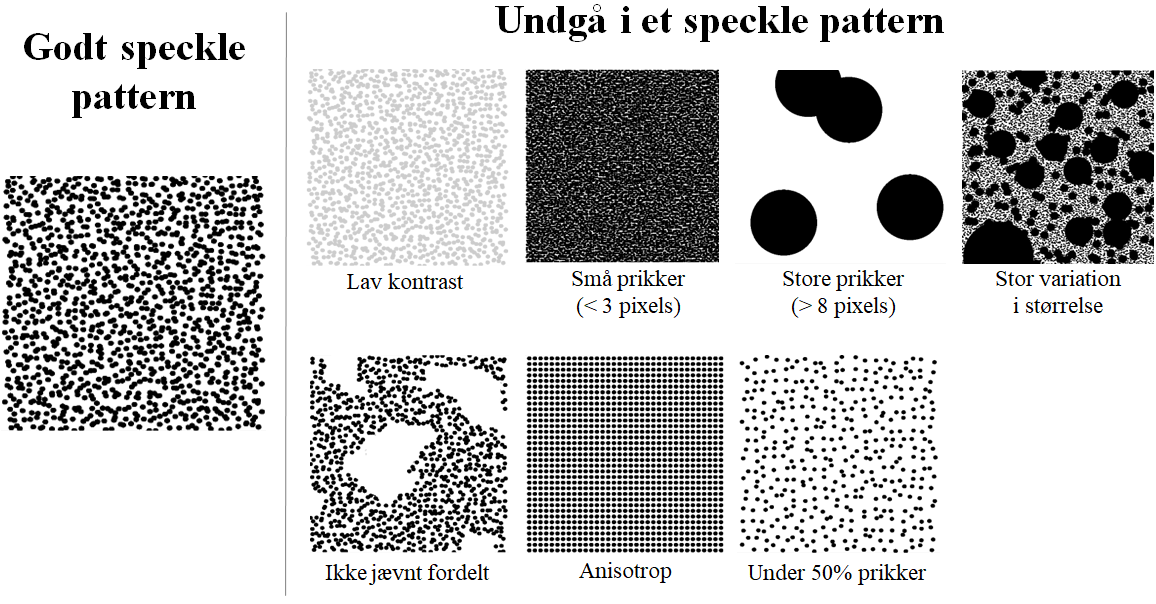
\includegraphics[width=0.9\textwidth]{Sections/2 Problemanalyse/Media/speckle pattern.png}
    \caption{Illustration af fejlkilder ved produktion af speckle pattern til DIC. Speckle pattern er genereret med software fra Correlated Solutions (\cite{CorrelatedSolutions2025SpeckleInc.})}
    \label{fig:godt speckle pattern}
\end{figure} \plainbreak{-0.4}

Figur \ref{fig:godt speckle pattern} illustrerer fejlkilder i speckle patterns, der mindsker præcisionen af DIC. Kriterierne for et godt speckle pattern er gældende for både 2D og 3D.


%-----
\subsubsection{Forblive på overfladen} \plainbreak{-0.4}
Det er nødvendigt, at prikkerne forbliver på og deformerer med overfladen af emnet der undersøges. Resultaterne af DIC er ikke retvisende, hvis prikkerne flytter sig uafhængigt af det undersøgte emne. Det er nødvendigt, at prikkerne flytter sig med emnet og ikke påvirker dets egenskaber. Derudover skal prikkerne ikke have tydelig ændring i gray-level eller geometri efter deformation.
(\cite{Dong2017ACorrelation} ; \cite{Zaya2023ApplicationReview}). \label{par:overfladen}



% --- Fremstilling ---
\plainbreak{2} \section{Fremstilling af speckle pattern} \label{Fremstilling af Speckle pattern}
Påføring af et speckle pattern i makroskala på en 2D flade, gøres på nuværende tidspunkt primært med enten spraydåse eller stempler. Det kan også gøres ved andre metoder såsom tusch eller midlertidige tatoveringer \parencite{Dong2017ACorrelation, Quino2021SpeckleEndurance}. Tidligere beskrevet i afsnit \ref{DIC afsnit}, afgrænses projektet til at skulle fremstille prikker i makroskala på $\geq \SI{0,1}{mm}$. Ved fremstilling af speckle pattern til DIC, ønskes det at parametrene er optimale, som beskrevet i afsnit \ref{Optimale speckle patterns}. 


\subsubsection{Spraydåser og Airbrush} \plainbreak{-.4}
Spraydåser og airbrushes producerer speckle patterns ved brug af trykluft til at blæse maling ud på en overflade. Spraymetoder er gode til at dække et område hurtigt og forholdsvist tilfældigt, idet malingens position kun kan bestemmes ved at ændre afstand til emnet, og retning som malingen udsendes i. Dette betyder, at malingen kan samles i større klumper, eller blive for sig selv i små pletter, der skaber unikke mønstrer, med stor variation i prikstørrelser. Dette kan være en udfordring, fordi der kan skabes for store mørke områder, eller kan ændre overfladetykkelsen. Derudover er airbrush og spraydåser begrænsede i, hvor store prikmønstrer de kan skabe. Dette overkommes ved at modificere på afstanden mellem emnet og dysen, dysens diameter, tryk i dysen og tykkelsen af væsken.\parencite{Dong2017ACorrelation, Quino2021SpeckleEndurance} 

Spraydåsen og airbrushen er ikke ens, og der er fordele ved, at bruge airbrush frem for spraydåser. Forskellen mellem airbrush og spraydåse kan ses på figur \ref{Spraymetode}, hvor de to billeder til venstre (a,b) er lavet med airbrush, og de to til højre (c,d) er udført med spraydåse. Her giver airbrushen et mere udspredt speckle pattern, og en større variation i prikstørrelse, som øger muligheden for unikke mønstre. Spraydåsen giver dog større risiko for afvigelse i prikstørrelserne, så der altid vil være prikker, der enten er for store eller for små til det ønskede speckle pattern. \parencite{Crammond2013SpeckleCorrelation}

\begin{figure}[H]
    \centering
    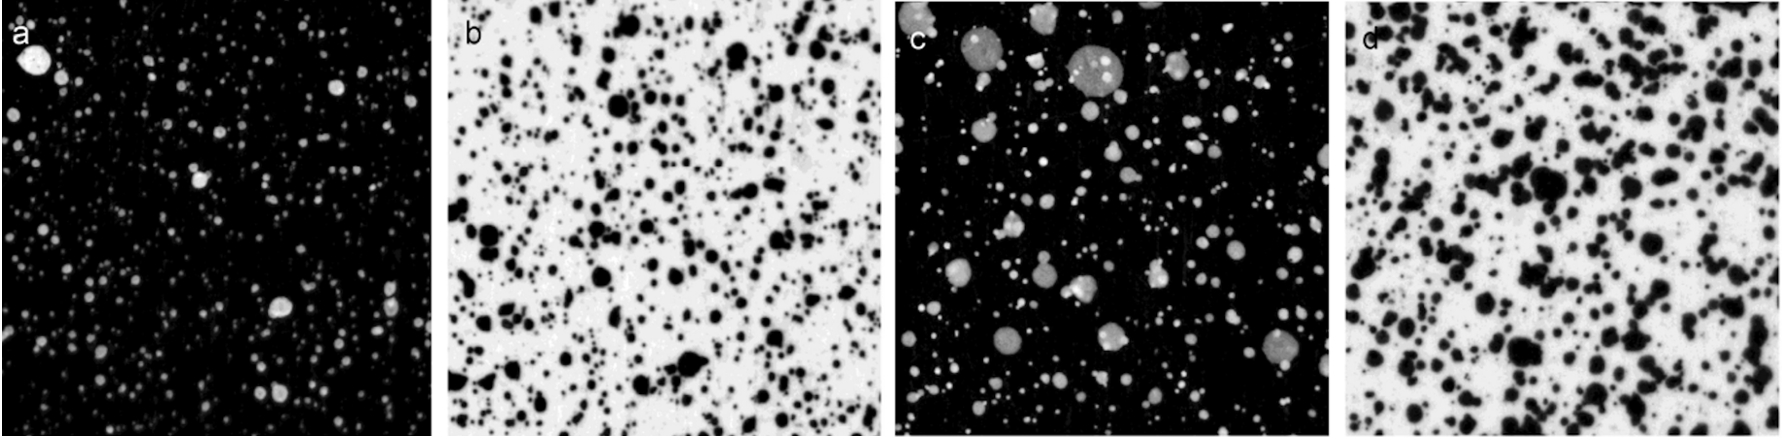
\includegraphics[width=1.0\linewidth]{Sections/2 Problemanalyse/Media/AirvsSprayinline.png}
    \caption{Speckle patterns med Airbrush og spraydåse. Her er a og b med Airbrush og c og d med Spraydåse \parencite{Crammond2013SpeckleCorrelation}}
    \label{Spraymetode}
\end{figure} \plainbreak{-0.5}


Spraydåsen er en priseffektiv metode til at påføre et  speckle pattern, hvor en spraydåse med 400 mL maling kan købes for 39,95kr. i Harald Nyborg (17.3.2025) \parencite{HaraldNyborg2025ColorWorksMat}. En airbrush har flere specialdele og kræver en kompressor for at virke, med det resultat, at den koster mere og anskaffe, modsat spraydåser \parencite{Dong2017ACorrelation}. Et airbrushsæt kan købes fra Amazon til omkring 600kr \parencite{TIMBERTECH2025Amazon.comAirbrush}.



\subsubsection{Stempel og stempelrulle} \plainbreak{-0.4}
Stemplet og stempelrullen er simple værktøjer til fremstilling af speckle pattern, da de ikke kræver andet end blæk at benytte. Anskaffelsesprisen er højere for stempelruller end airbrushes og spraydåser, hvor et sæt med 6 stempler, 6 ruller og noget blæk koster 2350\$ ($\simeq$ 16700 DKK, d. (25.2.2025)) hos Correlated Solutions. Eksempel på en stempelrulle kan ses i figur \ref{fig: Stempelrulle}. De størrelser der kommer i sættet fra Correlated Solutions, har stempelruller med prikdiametre fra $\SI{0,18}{mm}$ til $\SI{5,08}{mm}$, hvilket ved 1920:1080 opløsning, vil give en FOV fra $\SI{4,3}{cm}$ til $\SI{325}{cm}$. \parencite{CorrelatedSolutions2025VICCorrelation}

Stempler og rullerne virker ved, at blæk påføres deres overflade, som efterfølgende rulles over overfladen på emnet, hvor blækket overføres og efterlader et speckle pattern. Hvert stempel skaber mønstrer i en bestemt størrelse, hvilket begrænser antallet af forskellige emner og FOV'er det enkelt stempel kan bruges på, for at ramme 5-8 pixels pr. prik, som defineret i afsnit \ref{Speckle pattern}. \parencite{Dong2017ACorrelation}



\begin{figure}[H]
    \centering
    \begin{subfigure}{0.46\textwidth}
        \centering
        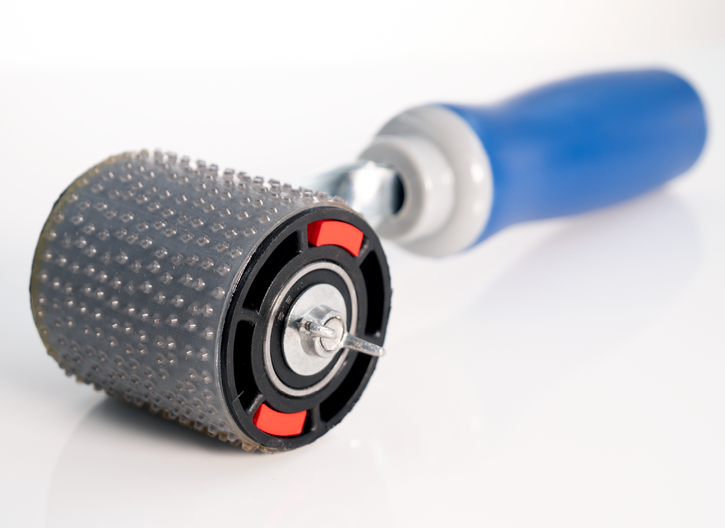
\includegraphics[width=.98\linewidth]{Sections/2 Problemanalyse/Media/Roller.png}
        \caption{Stempelrulle (\cite{CorrelatedSolutions2025VICCorrelation})}
        \label{fig: Stempelrulle}
    \end{subfigure}
    \begin{subfigure}{0.49\textwidth}
        \centering
         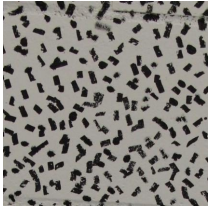
\includegraphics[width=0.7\linewidth]{Sections/2 Problemanalyse/Media/Tusch.png}
         \caption{Speckle pattern med overstregningstusch og lav densitet \parencite{HoseinSalmanpour2013PDFWalls}}
        \label{SpeckleTusch}
    \end{subfigure}
    \caption{}
    \label{fig:rulle og tush}
\end{figure} \plainbreak{-0.5}


\subsubsection{Tusch og andre skriveredskaber}  \plainbreak{-0.4}
En anden metode til påføring af speckle pattern, er tuscher og andre skriveredskaber, der sikre at prikkerne forbliver på overfladen af emnet under deformation. Et sæt med fire tuscher med en diameter på mellem \(\SI{0,1}{mm}\) og \(\SI{0,7}{mm}\) koster 13\$ ($\simeq$ 90 DKK, d. (6.3.2025)) \parencite{STAEDTLER2025Amazon.comTousch}. Metoden kræver, at prikkerne sættes manuelt én efter én på overfladen. Denne metode er tidskrævende, og kan være vanskeligt at opnå optimale parametre med, hvilket kan medføre fejlmålinger ved DIC, grundet mangel på nøjagtighed, som beskrevet i afsnit \ref{Speckle pattern}. Fordelen ved at prikkerne placeres manuelt er, at mønsteret ikke bliver isotropt. 
Det er et problem at prikkernes afstand mellem hinanden kan variere, da der kan skabes pletter, der er for store, eller områder med for lidt dækning af prikker, så der ikke kan observeres en deformation i de områder. Et eksempel på et speckle pattern tegnet med overstregningstusch kan ses i figur \ref{SpeckleTusch} \parencite{HoseinSalmanpour2013PDFWalls}. Usikkerheden ved metoden kan mindskes, hvis tiden der bruges på at sætte prikkerne øges. 





%Det er muligt at finde specielle tuscher eller kuglepenne, der er lavet med meget små spidser, så der kan laves prikker med en diameter på 100$\mu m$, som kan bruges i FOV'er helt ned til 2,2cm på langs (med en opløsning på 1920:1080).\parencite{Dong2017ACorrelation}.  her kan det blive et problem, da usikkerhederne kan medføre at der kommer klatter af ren farve eller andre fejl såsom mere farve end 70\% eller mindre end 50\%, som kan medføre fejlmålinger i DIC, grundet mangel på præcision (\ref{Speckle pattern}). Dette er muligt at undgå, hvis der bruges endnu længere tid på at gøre sine prikpositioner perfekte, som medfører mere tid brugt ved mindre skala.


\subsubsection{Midlertidig tatovering}  \plainbreak{-0.4}
En midlertidig tatovering, bruges til at overføre et bestemt mønster over på en flade. Dette fungerer ved, at der genereres et speckle pattern, som laserprintes ind på tatoveringspapiret. Herefter kan tatoveringen klistres på den ønskede overflade, hvorefter den vædes, så blækket overføres og forbliver på overfladen. Prisen på to A4 ark printbart papir til midlertidige tatoveringer koster 9.99\$ ($\simeq$ 69 DKK, d. 17.3.25) \parencite{SilhouetteAmerica2025TemporaryClearMEDIA-TATTOO-3T}. Det kræver en laserprinter, for at kunne printe en midlertidig tatovering, hvilket øger anskaffelsesprisen for denne metode.\parencite{Quino2021SpeckleEndurance}

\begin{comment}
    \begin{figure}[H]
    \centering
    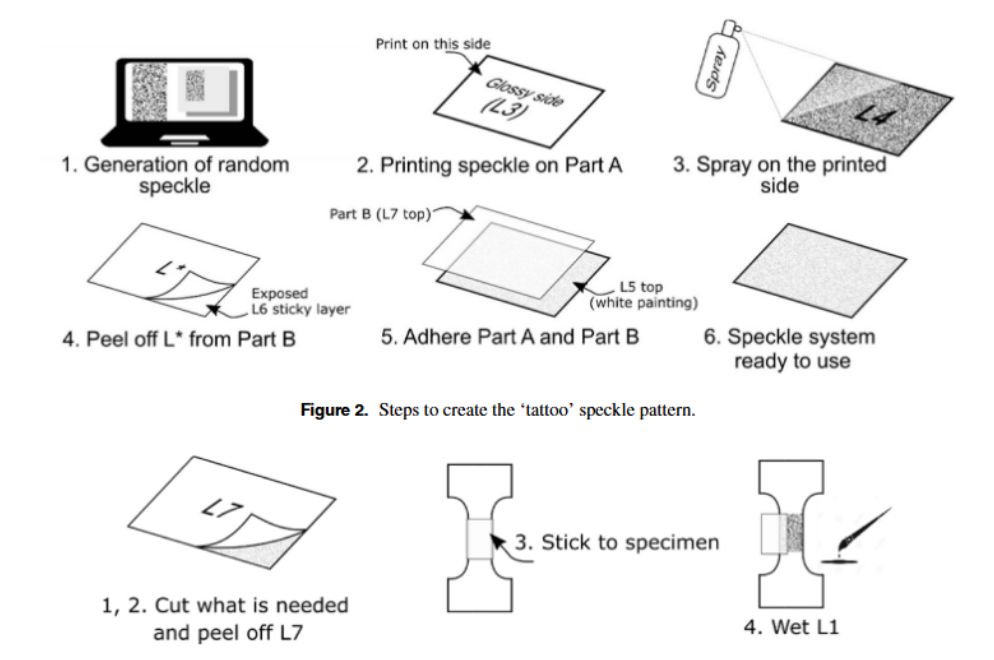
\includegraphics[width=0.8\linewidth]{Sections/2 Problemanalyse/Media/Temporary tattoo.png}
    \caption{Fremgangsmåde ved påføre af midlertidig tatovering med speckle pattern \parencite{Quino2021SpeckleEndurance}}
    \label{Midlertidigtatovering}
\end{figure}
\end{comment}



\subsection{Robotter til fremstilling af speckle pattern}  \label{Robotter til fremstilling af speckle pattern}
De nuværende produkter på markedet, der benyttes til fremstilling af speckle pattern, kræver manuelt arbejde og har varierende nøjagtighed i densitet og størrelse af prikker. På baggrund heraf vurderes det, at brugen af robotter til fremstilling af speckle patterns kan automatisere processen og har potentiale for at øge genskabeligheden. Sådan en løsning muliggør altå at der kan laves mere ensartetede prøver af flere af samme emnetype og dermed øges nøjagtigheden af DIC.


%Den mest brugte metode er spraydåsen, altså spraydåser og airbrush \parencite{Dong2017ACorrelation, Quino2021SpeckleEndurance}. Det vil altså være optimalt at kunne lave en løsning, der er mere effektiv end denne løsning. Spraymetoden er optimeret i forhold til pris og påføringshastighed, hvor spraydåser er engangsforbrug, og airbrush kan genbruges, men kræver en kompressor og maling. Det er derfor svært at slå disse to i pris og påføringshastighed, og det er derfor et ønske at lave et bedre produkt, som er bedre til at danne speckle patterns end spraymetoden er.

%En af de ting som spraymetoden ikke er god til, er at den er lidt for tilfældig, og store mængder maling kan samle sig på samme sted. Det vil derfor være et ønske, at løsningen skal kunne skabe et præcist mønster pålideligt, hvilket indebærer at der ikke skabes prikker mindre end 3 og større end 7 pixels (\ref{Speckle pattern}).

 

% --- Robotter --- 
\plainbreak{2} \section{Robotter} \label{Robotter}

Robotter er et mekanisk eller mekatronisk system, der selvstændigt eller delvist selvstændigt kan udføre én eller flere handlinger. Systemet styres typisk af en programmerbar styreenhed, der enten kan følge forudbestemte instruktioner eller tilpasse sin adfærd baseret på sensorinput. Robotter anvendes ofte til at automatisere opgaver, hvor der er krav om gentagelse, præcision eller effektivitet, og hvor manuel udførelse kan være forbundet med variation eller upræcise resultater. En robot består grundlæggende af flere integrerede systemer, der sammen muliggør kontrol over bevægelser og handlinger. Det mekaniske system danner grundstrukturen og kan være enten stationært eller bevægeligt, afhængigt af hvordan det skal interagere med emnet. \parencite{TextbookofRobotics}

%På baggrund af afsnit \ref{Fremstilling af Speckle pattern}, vurderes det, at robotter med fordel kan anvendes til fremstilling af speckle patterns. Manuelle metoder til at påføre speckle patterns, som for eksempel brug af airbrush eller tusch, kan føre til variationer i kvaliteten af mønstret. Disse variationer kan have en negativ indvirkning på nøjagtigheden og reproducerbarheden af målinger i DIC. Ved at anvende en robot forventes det, at påføringsprocessen kan standardiseres, hvilket sikrer en mere ensartet kvalitet og dermed mere pålidelige måleresultater.

%En vigtig del af robotten er påføringsmekanismen, som kan variere alt efter metode. Den kan for eksempel være baseret på sprøjteteknikker som airbrush, trykbaserede metoder som stempling eller andre teknologier, der overfører et prædefineret mønster, eksempelvis via print eller midlertidige tatoveringer. \parencite{TextbookofRobotics}

For at opnå nøjagtige bevægelser indgår der typisk sensorer i robotløsninger, der kontroller, at den teoretiske bevægelse også er udført i virkeligheden. Disse sensorer kan være kameraer, afstandsmålere eller kraftmålere, som giver systemet mulighed for at opdage afvigelser. Sensorerne sender data tilbage til styreenheden, som kan være en mikrocontroller eller computer, der i realtid kan behandle dataen og foretager de nødvendige justeringer. Dette samarbejde mellem sensorer, styreenhed og mekaniske komponenter er afgørende for, at kunne udføre de ønskede bevægelser og handlinger med nøjagtighed. \parencite{BasicsofRobotics}

Hvilken type robot, der kan være velegnet til opgaven, afhænger af en række forskellige faktorer. Eksempelvis kan størrelsen og geometrien på de testemner, der arbejdes med, have indflydelse på, hvordan systemet bør være udformet og bevæge sig i forhold til emnet. Desuden kan der være forskelle i, hvordan forskellige løsninger håndterer bevægelse, positionering og interaktion med omgivelserne. Derfor er det relevant at undersøge, hvilke forskellige typer af robotter der findes, og hvordan de adskiller sig fra hinanden.
\plainbreak{1}\subsection{Robottyper} \label{Robottyper}
Robotter kan klassificeres på forskellige måder afhængigt af den opgave de udfører, miljøet de gør det i, design og autonominiveau. Af de kategorier der er beskrevet i ISO 8373:2021 \parencite{ISO2021ISOVocabulary} og \cite{IFR2023World2023} er der to relevante kategorier for projektet. Desuden er printere og 3D FDM printere også inkluderet, da de udfører lignende opgaver.

\textbf{Industrirobotter} er automatiserede og programmerbare maskiner, der bruges i industrielle miljøer til opgaver såsom samling, svejsning og malerarbejde \parencite{IFR2023World2023}. Industrielle robotter kommer i alle størrelser, men kræver, til forskel fra de andre kategorier, særlig infrastruktur omkring dem. Det kan fx være indhegninger for robot arme, som vist på figur \ref{fig:irb7710pic}. De skal dermed ikke tage højde for mennesker, og bruges ofte til at udføre opgaver, hvor det er for dyrt eller farligt at ansætte folk \parencite{ABB2023IRBSeries, ISO2021ISOVocabulary}. 

\begin{figure}[H]
    \centering
    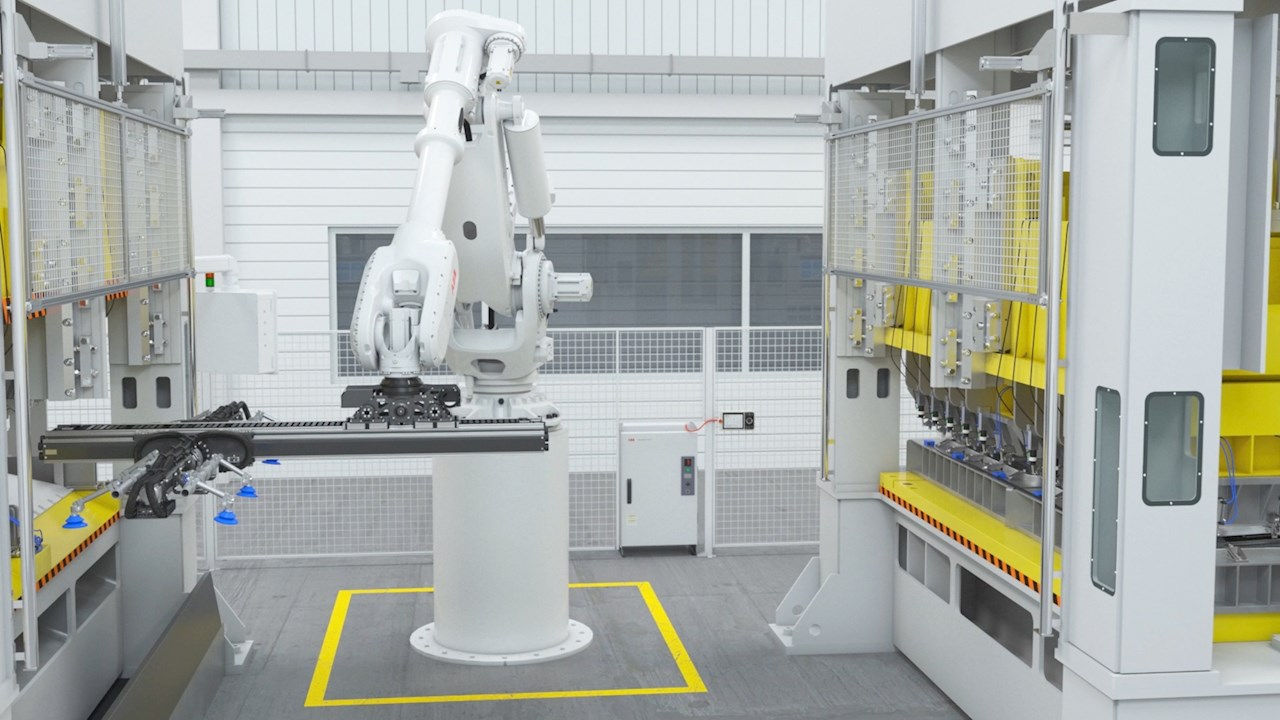
\includegraphics[width=0.6
    \textwidth]{Sections/2 Problemanalyse/Media/irb7710.jpg}
    \caption{IRB-7710 robotarm fra ABB \parencite{ABB2023IRBSeries}}
    \label{fig:irb7710pic}
\end{figure} \plainbreak{-0.5}
\textit{Eksempel:} ABB's IRB-robotter, serien indeholder mange forskellige størrelser af robotter. På figur \ref{fig:irb7710pic} ses model 7710, som er i den store ende og har en løftekapacitet på op til \SI{500}{kg}. På figuren er den sat op til at flytte store plader fra en stor maskine til en anden, robotten er praktisk her, da den kan løfte pladen fra midten af den ene maskine, og placere den i midten af den anden.
    
\textbf{Collaborative Robots (Cobots)} er designet til at arbejde sikkert sammen med mennesker i fælles arbejdsområder. De er ofte udstyret med sensorer og avancerede kontrolsystemer for at sikre at de kan koeksistere sikkert med mennesker \parencite{IFR2023World2023}. Her er sikkerhed altså en meget høj prioritet. Til forskel fra Servicerobotter er denne type ofte mere generaliserede og designet til at kunne arbejde sammen med mennesker, ikke blot i samme miljø.

\begin{figure}[H]
    \centering
    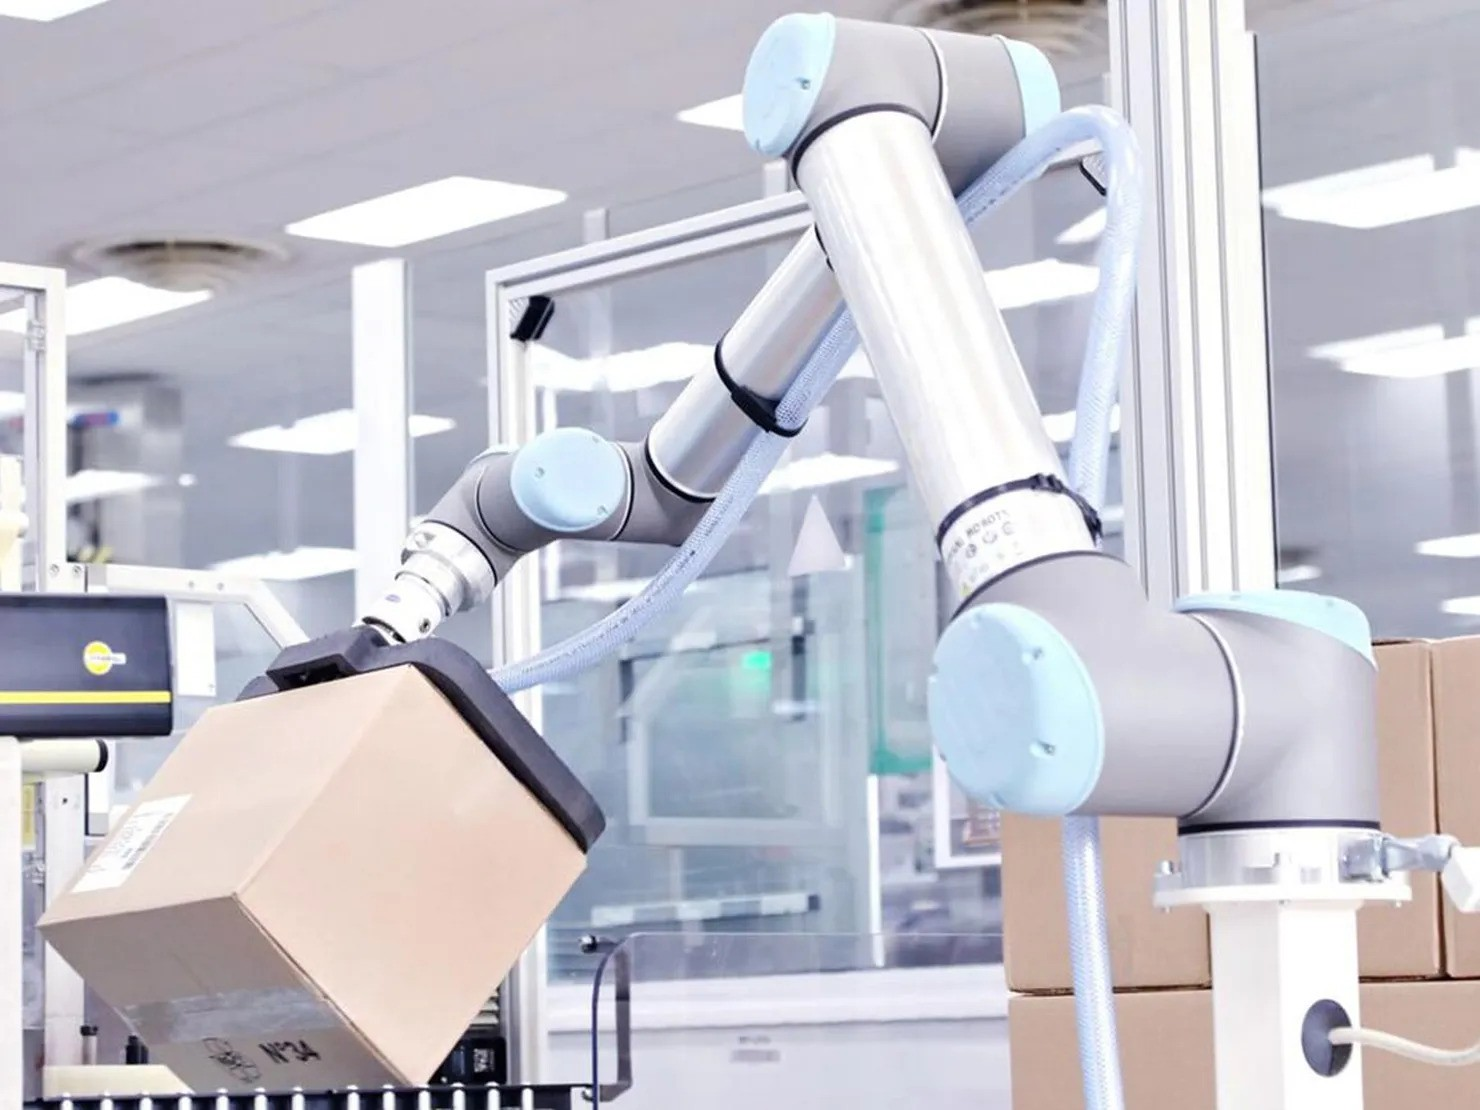
\includegraphics[width=0.5\linewidth]{Sections/2 Problemanalyse/Media/URrobot.jpg}
    \caption{UR5, et letvægt Cobot lavet i Danmark \parencite{2023URSeries}}
    \label{fig:ur5pic}
\end{figure} \plainbreak{-0.5}

\textit{Eksempel:} Universal Robots' UR-serie \parencite{2023URSeries}. Designet til at være flexible, billig og let. Primært tænkt til at samle op, flytte og placere. Fx kan den placere en del foran et mennesker, der kan udføre noget arbejde, hvorefter UR5 kan flytte den væk igen. Cobots bruges altså til at automatisere simple handlinger hvorimod mennesker stadig udføre mere kompliceret arbejde.

\textbf{Printere} er en type maskine, hvor et printhoved bevæger sig hen over en overflade for at afsætte små dråber væske i et præcist mønster. Systemet består typisk af en mekanisk struktur, der styrer printhovedets bevægelser i én retning, mens underlaget enten er stationært eller bevæges i en vinkelret retning. Bevægelsen kontrolleres af motorer, som sikrer en jævn og præcis føring, hvilket gør det muligt at opnå en ensartet fordeling af materialet på overfladen. Afhængigt af konstruktionen kan nogle systemer også bevæge printhovedet i begge retninger og på den måde optimere hastigheden og effektiviteten.\parencite{Delaney2009InkjetProteins} 

\begin{figure}[H]
    \centering
    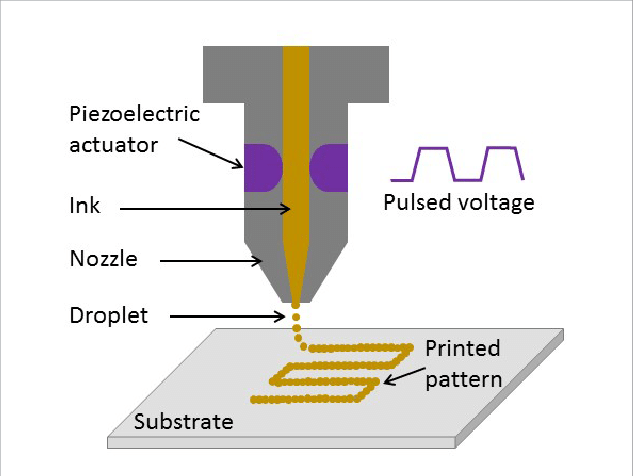
\includegraphics[width=0.5\linewidth]{Sections/2 Problemanalyse/Media/inkjet.png}
    \caption{Illustration af hvordan en Inkjet printer fungere \parencite{Long2025AOptimizations}}
    \label{fig: Inkjet}
\end{figure} \plainbreak{-0.5}

Inkjet-printere anvender dyser, der sprøjter væske ud som små dråber. Størrelsen på disse dråber og afstanden mellem dem bestemmes af både dysens udformning og systemets præstationsniveau, se figur \ref{fig: Inkjet}. Printhovedet kan tilpasses til at håndtere forskellige væsketyper, hvilket gør teknologien fleksibel i forhold til materialevalg. Systemet er primært designet til at arbejde på plane eller næsten plane overflader, da det kræver en ensartet afstand mellem printhovedet og emnet for at sikre korrekt afsætning af materialet.\parencite{Delaney2009InkjetProteins} 

Inkjet-printers bevægelsessystemer er karakteriseret ved høj nøjagtighed og genskabelighed, hvilket gør dem velegnede til opgaver, hvor præcis materialepositionering er nødvendigt. Systemet er ofte simpelt opbygget og kan tilpasse forskellige størrelser afhængigt af anvendelsen. Selvom inkjet-printere ofte anvendes til at printe tekst eller billeder på papir, kan teknologien også tilpasses andre formål, hvor præcis placering af små dråber eller partikler er nødvendigt.

%De andre printerteknologier, laser og termisk, kan allerede nu kasseres da laserprintere vil varme emnet op, og dermed kan ændre emnets egenskaber og termiske printer kun virker da papiret er varmereaktivt. De er derfor ikke relevante.

\textbf{FDM 3D Printere} bruges ofte med et standard kartesisk bevægelsessystem.  Det kartesiske bevægelsessystem for 3D-printeren er kendetegnet ved, at elmotorer kontrollerer bevægelse langs tre akser, x-, y- og z aksen, se figur \ref{fig:3D printer}.

\begin{figure} [H]
    \centering
    \includegraphics[width=0.5\linewidth]{Sections/2 Problemanalyse/Media/3D printer bevægelse.png}
    \caption{3D printer illustration. \parencite{Mueller20203DDraft}. }
    \label{fig:3D printer}
\end{figure}\plainbreak{-0.5}

 De er ofte lavet med bælter eller med en ledeskrue der kan føre printerhovedet i de tre retninger. Dette vil også være en mulig måde at lave en robotbevægelse, til påføring af speckle patterns, på en 2D overflade. \parencite{Billington20243DOverview}
\plainbreak{1} \input{Sections/2 Problemanalyse/4.2 Robotbevægelser}
